%-------------------------
% Resume in Latex
% Author : Matty
% Based on: https://github.com/jakegut/resume (which was itself based on https://github.com/sb2nov/resume)
% License : MIT
%------------------------

\documentclass[letterpaper,11pt]{article}
\usepackage{graphicx}
\usepackage{latexsym}
\usepackage[empty]{fullpage}
\usepackage{titlesec}
\usepackage{marvosym}
\usepackage[usenames,dvipsnames]{color}
\usepackage{verbatim}
\usepackage{enumitem}
\usepackage[hidelinks]{hyperref}
\usepackage{fancyhdr}
\usepackage[english]{babel}
\usepackage{tabularx}
\usepackage{xcolor}
\usepackage{fontawesome5}

\input{glyphtounicode}

% -------------------- FONT OPTIONS --------------------
% sans-serif
% \usepackage[sfdefault]{roboto}
% \usepackage[sfdefault]{noto-sans}
% serif
% \usepackage{charter}
% Set custom font sizes


\pagestyle{fancy}
\fancyhf{} % clear all header and footer fields
\fancyfoot{}
\renewcommand{\headrulewidth}{0pt}
\renewcommand{\footrulewidth}{0pt}

% Adjust margins
\addtolength{\oddsidemargin}{-0.5in}
\addtolength{\evensidemargin}{-0.5in}
\addtolength{\textwidth}{1in}
\addtolength{\topmargin}{-1in} % Default was -.5in
\addtolength{\textheight}{1.0in}

\urlstyle{same}

\raggedbottom
\raggedright
\setlength{\tabcolsep}{0in}

% Section formatting
\titleformat{\section}{
  \vspace{-5pt}\scshape\raggedright\large
}{}{0em}{}[\color{black}\titlerule \vspace{-5pt}]

% Subsection formatting
\titleformat{\subsection}{
  \vspace{-4pt}\scshape\raggedright\large
}{\hspace{-.15in}}{0em}{}[\color{black}\vspace{-8pt}]

% Ensure that generate pdf is machine readable/ATS parsable
\pdfgentounicode=1

% -------------------- CUSTOM COMMANDS --------------------
\newcommand{\resumeItem}[1]{
  \item\small{
    {#1 \vspace{-2pt}}
  }
}

\newcommand{\resumeSubheading}[4]{
  \vspace{-2pt}\item
    \begin{tabular*}{0.97\textwidth}[t]{l@{\extracolsep{\fill}}r}
      \textbf{#1} & #2 \\
      \textit{\small#3} & \textit{\small #4} \\
    \end{tabular*}\vspace{-7pt}
}

\newcommand{\resumeSubSubheading}[2]{
    \item
    \begin{tabular*}{0.97\textwidth}{l@{\extracolsep{\fill}}r}
      \textit{\small#1} & \textit{\small #2} \\
    \end{tabular*}\vspace{-7pt}
}

\newcommand{\resumeProjectHeading}[2]{
    \item
    \begin{tabular*}{0.97\textwidth}{l@{\extracolsep{\fill}}r}
      \small#1 & #2 \\
    \end{tabular*}\vspace{-7pt}
}

\newcommand{\resumeSubItem}[1]{\resumeItem{#1}\vspace{-4pt}}
\newcommand{\resumeSubHeadingListStart}{\begin{itemize}[leftmargin=0.15in, label={}]}
\newcommand{\resumeSubHeadingListEnd}{\end{itemize}}
\newcommand{\resumeItemListStart}{\begin{itemize}}
\newcommand{\resumeItemListEnd}{\end{itemize}\vspace{-5pt}}

\renewcommand\labelitemii{$\vcenter{\hbox{\tiny$\bullet$}}$}

\setlength{\footskip}{4.08003pt}

% -------------------- START OF DOCUMENT --------------------
\begin{document}


% -------------------- HEADING--------------------
\begin{flushright}
  % \vspace{-4pt}
  \color{gray}
  \item
  Last Updated on November 31st, 2024
\end{flushright}

\vspace{-5pt}

\begin{center}
    \begin{tabular}{l l}
    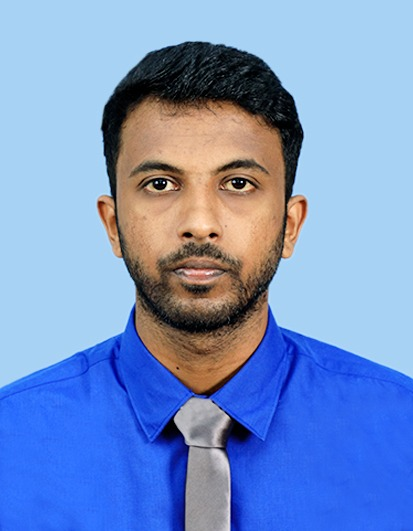
\includegraphics[width=3.5cm, height=4.5cm]{kajan.jpeg}& 

    \end{tabular}
    \textbf{\Huge \scshape Kunendran Kajavathanan} \\ 
    \vspace{8pt}
    \small 
    \faIcon{github}
    \href{https://github.com/Kajavathanan}{\underline{github.com/Kajavathanan}} $  $
    \faIcon{code}
    % \href{https://www.mattydoe.com} portfolio website
    % {\underline{mattydoe.com}} $  $
    % \faIcon{linkedin}
    \href{https://www.linkedin.com/in/kajavathanan-kunendran}{\underline{linkedin.com/in/kajavathanan}} $  $
    \faIcon{envelope}
    \href{mailto:kajavathanankunendran@gmail.com}
    {\underline{kajavathanankunendran@gmail.com}}
\end{center}

% -------------------- EDUCATION --------------------
\section{Education}
  \resumeSubHeadingListStart
<<<<<<< HEAD
=======
  
    \resumeSubheading
      {Institute of Technology, University of Moratuwa}{Mar. 2020 - Mar. 2024}
      {Diploma in Electronic and Telecommunication}{Current GPA: 3.46/4.0} 
>>>>>>> 550d09fee1490506266e7f8266306cc4f68e9e2c
      
    \resumeSubheading
      {University of the West of England\footnotesize{}}{May. 2023 -- Present }
      {B.Eng(Hons) in Electrical and Electronic Engineering}{}

    \resumeSubheading
      {Institute of Technology, University of Moratuwa}{Mar 2020 -Mar 2024}
      {Diploma in Electronic and Telecommunication Engineering}{Current GPA: 3.39/4.0}  

    \vspace{-8pt} 

    \subsection{Certifications}
      \textbf{SystemVerilog for ASIC/FPGA Design and Simulation :} Skill Surf\\
      \textbf{Machine Learning Engineer- Stage 1 :} SLIIT \\
      \textbf{Microcontroller based Embedded System Design :} University of Moratuwa
      

  \resumeSubHeadingListEnd

% -------------------- SKILLS --------------------
\section{Skills}
 \begin{itemize}[leftmargin=0.15in, label={}]
    \small{\item{

     \textbf{Expertise}{: Design Verification(UVM), RTL Design} \\
    
     \textbf{Programming Languages}{: C++, SystemVerilog, Tcl } \\
     
     \textbf{Protocols}{: AXI, UART, PCIE, APB, AHB} \\

     \textbf{Tools and Framework}{: Siemens Questa, Vivado, Vitis, Git/GitHub} \\
     
     \textbf{Languages}{: Tamil-native, English-Excellent} \\
     
     
     
    }}
 \end{itemize}

% -------------------- PROJECTS --------------------
\section{Projects}
    \resumeSubHeadingListStart

        \resumeProjectHeading
        {\textbf{Single-Cycle RISC-V Processor Design} $|$ \footnotesize\emph{SystemVerilog, Questa,  Git, VS Code}} {Jul. 2024}
        \resumeItemListStart
          \resumeItem{Implemented Risc-V instructionset Architecture, Including logical and Memory location instruction.}
          \resumeItem{Developed control logic to manage instruction execution within a single clock cycle.}
          \resumeItem{Developed a comprehensive Testbench in System Verilog to simulate and Verify the Design.}
        \resumeItemListEnd

        \resumeProjectHeading
        {\textbf{FPGA-Based Block RAM Design and Implementation Project} $|$ \footnotesize\emph{ Vivado, Vitis, Questa}} {May. 2024}
        \resumeItemListStart
            \resumeItem{FPGA-based project focused on the design, implementation, and verification of Block RAM using \\Xilinx tools.}
            \resumeItem{Used Zybo-Z7 board to implement the design and Used Gtk term to read Data from Ports.}
            \resumeItem{Implemented UART communication to interact with the FPGA, enabling real-time data reading and \\writing via a serial terminal.}
            % \resumeItem{Optimized UX e.g. sound design, food drop timing, supplied saturation level, and addressed potential workarounds}
        \resumeItemListEnd
    
        \resumeProjectHeading
        {\textbf{UVM Verification of SBE Decoder with AXI4-Stream Agent} $|$ \footnotesize\emph{System Verilog, Questa Git, VS Code}}{Feb. 2024 }
        \resumeItemListStart
            \resumeItem{Created a UVM-compliant AXIS agent with AXIS interface capabilities.}
            \resumeItem{Conducted thorough UVM verification of the SBE decoder module, ensuring robust performance \\ and reliability.}
            % \resumeItem{Collaborated with livestreamers to get feedback and suggested features}
            % \resumeItem{Solved problems relating to asynchronous tasks}
          \resumeItemListEnd

        \resumeProjectHeading
        {\textbf{UVM Verification of Single-Port and Dual-Port RAM} $|$ \footnotesize\emph{SystemVerilog, Questa,  Git, VS Code}}{Nov. 2023}
        \resumeItemListStart
            \resumeItem{UVM verification of single-port and dual-port RAM modules, addressing write collision issues.}
            \resumeItem{Utilized OOP to enhance the UVM testbench for robust and efficient verification.}
            \resumeItem{This project demonstrated strong expertise in advanced verification techniques and contributed \\ to reliable memory design solutions.}
          \resumeItemListEnd    
          
      
          
    \resumeSubHeadingListEnd

    \newpage % Starts a new page
    \null
    \vspace{1.5cm} % Adjust the spacing as needed
% -------------------- EXPERIENCE --------------------
  
\section{Work Experience}
  \resumeSubHeadingListStart
          \resumeProjectHeading
          {\textbf{Accelr} $|$ \footnotesize\emph{Associate Electronic Engineer}}{March. 2024 -- Sep 2024}
          \resumeItemListStart
            \resumeItem{Hands-on experience in UVM verification, designed RTL for basic architectures, and expanded \\ my knowledge of the RISC-V architecture.}
            \resumeItem{Worked with Hardware Accelerator Team to Verifiy the Designed SBE Decoder.This included \\ creating test cases and running simulations to ensure the decoder functioned correctly and\\met performance requirements.}
            \resumeItem{Conducted research and development on PCIe protocol delivering presentations to fellow engineers to \\enhance their understanding of high-speed communication standards.}
            
        \resumeItemListEnd
          

          \resumeProjectHeading
          {\textbf{Accelr} $|$ \footnotesize\emph{Electronic Intern}}{Sep. 2023 -- March. 2024}
          % \small{Routinely tutor K--12 students in math, coding, etc.}
          \resumeItemListStart
            \resumeItem{Hands-on experience in UVM verification, designed RTL for basic architectures, and expanded \\ my knowledge of the RISC-V architecture.}
            \resumeItem{Worked with RTL Design Engineers to Design a UDP Parser and Designed multiple versions to find effficient \\way to produce results.}
            % \resumeItem{Optimized UX e.g. sound design, food drop timing, supplied saturation level, and addressed potential workarounds}
        \resumeItemListEnd

        \resumeProjectHeading
          {\textbf{Airport and Aviation, Srilanka} $|$ \footnotesize\emph{Electronic Intern}}{March. 2023 -- Sep. 2023}
          \resumeItemListStart
            \resumeItem{Assisting in the design and testing of electronic systems related to air safety and aviation electronics.\\Involved in designing voice communication system for Ratmalana Airport}
            \resumeItem{Designed Redundant voice communication system with the engineering team.Which composed of \\Amplifiers and push to talk features works in specific frequencies.}
            \resumeItem{Optimize the Design of Arduino based GPS Clock used in Jaffna International Airpot which helped\\ overcome the heating issues in voltage Regulators and provided support to automating Recordings of \\ Air traffic controllers with python scripts.}
        \resumeItemListEnd
          % {\small{Assisting in the design and testing of electronic systems related to air safety and aviation electronics.Involved in designing voice communication system for Ratmalana Airport.}}

          
          % {\small{Earned an award for philanthropic hours spent, still giving away 100 stocked backpacks a year}}
          
        % \subsection{Hobbies}
          
        %   \resumeProjectHeading
        %   {\textbf{Playing the Drums}\vspace{8pt}}{2013 -- 2019}
        %   {\small{Played the drums in symphonic, jazz, and marching bands}}

        %   \resumeProjectHeading
        %   {\textbf{3\textsuperscript{rd} Place Time Keeping Challenge Championship \footnotesize{(Time Keeping Assocation)}}\vspace{8pt}}{Feb. 2022 -- May 2022}
        %   {\small{Won \$1500 nationally competing against high school students in counting seconds and minutes}}
          
    \resumeSubHeadingListEnd 

\end{document}
<<<<<<< HEAD



% Ensuring all equipment and products meet health and safety regulations.
% Observing existing processes and making recommendations for improvement.
% Developing effective maintenance, testing, and quality control procedures.
% Showing initiative and keeping up with advancements in Electronics.
% Representing the company at conferences and delivering presentations if required.
% Monitoring processes, systems, and staff, and punctually identifying problems.
% Establishing relationships with staff, vendors, suppliers, and other professionals in the field.
% Writing specifications, instructions, reports, and handling other required administrative duties.
% Electronics Engineer Requirements:
% Bachelor's degree in Engineering or similar.
% Master's degree preferable.
% A relevant license may be required.
% Practical experience with design software.
% Experience in design recommended.
% Excellent problem-solving and troubleshooting skills.
% Strong written, verbal, and telephonic communication skills.
% Excellent research and interpersonal skills.
% Strong analytical skills.
% Willingness to work overtime if required.
=======
>>>>>>> 550d09fee1490506266e7f8266306cc4f68e9e2c
